\documentclass[12pt]{article}
\usepackage[T1]{fontenc}
\usepackage[utf8]{inputenc}
\usepackage[polish]{babel}
\usepackage{graphicx}
\usepackage{amsfonts}
\usepackage{booktabs}
\usepackage{array}
\usepackage{hyperref}
\usepackage[section]{placeins}

\setlength{\textheight}{22cm}

\title{{\bf Zadanie nr 3 -- Klasyfikacja obrazów kart do gry\\przy użyciu konwolucyjnych sieci neuronowych}\linebreak
Techniki Inteligentnej Analizy Danych}
\author{Nikodem Nowak, 251598 \and Bartosz Kołaciński, 251554}
\date{2026-05-06}

\begin{document}
\clearpage\maketitle
\thispagestyle{empty}
\newpage
\tableofcontents
\thispagestyle{empty}
\newpage
\setcounter{page}{1}

%%%%%%%%%%%%%%%%%%%%%%%%%%%%%%%%%%%%%%%%%%%%%%%%%%%%%%%%%%%%%%%%%%%%%%%%%%%%%%%%
\section{Cel zadania}

Celem zadania było zaprojektowanie, wytrenowanie oraz porównanie skuteczności kilku architektur konwolucyjnych sieci neuronowych w problemie klasyfikacji obrazów. Zgodnie z wymogami zadania na ocenę 5 (treść instrukcji~\cite{wikamp_zad3}) przygotowano następujący zakres prac:

\begin{itemize}
  \item porównanie pięciu różnych modeli sieci konwolucyjnych: MobileNetV2~\cite{mobilenetv2}, ResNet50~\cite{resnet}, EfficientNetB0~\cite{efficientnet}, InceptionV3~\cite{inceptionv3} oraz VGG16~\cite{vgg};
  \item analiza wpływu proporcji podziału zbioru na uczący i testowy: 50/50, 60/40, 70/30, 80/20 oraz 90/10;
  \item ewaluacja jakości klasyfikacji za pomocą macierzy pomyłek oraz miar accuracy, precision, recall i F1 obliczanych w wariantach \textit{macro};
  \item przedstawienie krzywej ROC oraz wartości AUC w wariancie \textit{one-vs-rest} (OvR), z wykorzystaniem modułu \texttt{scikit-learn}~\cite{sklearn}.
\end{itemize}

Łącznie wykonano $5 \cdot 5 = 25$ niezależnych eksperymentów treningowych.

%%%%%%%%%%%%%%%%%%%%%%%%%%%%%%%%%%%%%%%%%%%%%%%%%%%%%%%%%%%%%%%%%%%%%%%%%%%%%%%%
\section{Wstęp teoretyczny}

\subsection{Konwolucyjne sieci neuronowe}

Konwolucyjne sieci neuronowe (CNN) stanowią dominujące podejście w klasyfikacji obrazów od momentu publikacji architektury AlexNet w 2012 r. Ich kluczową cechą jest hierarchiczny ekstraktor cech: wczesne warstwy konwolucyjne uczą się rozpoznawać proste wzorce (krawędzie, gradienty kolorów), warstwy środkowe tekstury i części obiektów, a najgłębsze całe obiekty oraz ich kompozycje~\cite{vgg}.

Każda z wykorzystanych w pracy architektur reprezentuje odrębny pomysł na efektywną budowę takiego ekstraktora:

\begin{itemize}
  \item {\bf VGG16}~\cite{vgg} -- klasyczna, "płaska" architektura zbudowana z powtarzających się bloków \texttt{Conv-Conv-Pool}; około 138~mln parametrów (z czego znaczna większość przypada na warstwy w pełni połączone, które w naszym podejściu zostały zastąpione własną głową);
  \item {\bf InceptionV3}~\cite{inceptionv3} -- wykorzystuje moduły Inception, w których wyniki konwolucji $1 \times 1$, $3 \times 3$ i $5 \times 5$ działających równolegle są łączone, co umożliwia analizę cech w różnych skalach przestrzennych;
  \item {\bf ResNet50}~\cite{resnet} -- wprowadza połączenia rezydualne (\textit{skip connections}) postaci $f(x) + x$, dzięki którym możliwe stało się trenowanie sieci o dziesiątkach warstw bez problemu zanikającego gradientu;
  \item {\bf MobileNetV2}~\cite{mobilenetv2} -- zoptymalizowana pod urządzenia mobilne (3{,}5~mln parametrów); kluczową techniką są \textit{depthwise separable convolutions}, rozkładające standardową konwolucję na dwie tańsze obliczeniowo operacje;
  \item {\bf EfficientNetB0}~\cite{efficientnet} -- wprowadza \textit{compound scaling}, czyli matematycznie wyznaczone optymalne proporcje skalowania głębokości, szerokości i rozdzielczości wejścia.
\end{itemize}

\subsection{Uczenie z transferem (transfer learning)}

W zadaniu klasyfikacji 14 typów kart dysponowaliśmy zbiorem o stosunkowo niewielkiej liczebności (8154 obrazy). Trening sieci od podstaw (z losowo zainicjalizowanymi wagami) na takim zbiorze prowadziłby do dramatycznego niedouczenia, gdyż współczesne CNN posiadają dziesiątki milionów parametrów. Rozwiązaniem stosowanym powszechnie w tej sytuacji jest {\bf transfer learning}~\cite{transfer_yosinski}, polegający na wykorzystaniu wag wytrenowanych wcześniej na dużym, ogólnym zbiorze danych -- tutaj ImageNet~\cite{imagenet} (1{,}2~mln obrazów, 1000 klas).

W naszym pipeline każdy z wymienionych modeli był ładowany z wagami z ImageNetu, a następnie modyfikowany w następujący sposób:
\begin{enumerate}
  \item odcięto oryginalną warstwę klasyfikującą (parametr \texttt{include\_top=False});
  \item zastosowano \textit{global average pooling}, redukując mapy cech do pojedynczego wektora;
  \item dodano warstwę \texttt{Dropout}~\cite{dropout} z prawdopodobieństwem 0{,}5 (regularyzacja przeciw przeuczeniu);
  \item dodano warstwę \texttt{Dense} z 14 neuronami i aktywacją \textit{softmax} (jedna na każdy typ karty).
\end{enumerate}

\subsection{Trening dwufazowy}

Ze względu na różnicę dziedzinową między ImageNetem (zdjęcia obiektów codziennych) a obrazami kart (schematyczne, płaskie wzory), zastosowano dwufazowy schemat treningu:

\begin{enumerate}
  \item {\bf Faza 1} -- "zamrożony" backbone (\texttt{trainable=False}); trenowane są wyłącznie wagi własnej głowy klasyfikującej. Optymalizator Adam~\cite{adam} z $\eta = 10^{-3}$, do 8 epok;
  \item {\bf Faza 2} -- odmrożenie 1/3 najwyższych warstw backbone'u (warstwy bliżej wyjścia są bardziej specyficzne dla domeny i wymagają dostrojenia, niższe pozostają niezmienione). Warstwy \texttt{BatchNormalization}~\cite{batchnorm} celowo pozostawiono w trybie inference, aby uniknąć destabilizacji statystyk populacji obliczonych na ImageNecie. Optymalizator Adam z $\eta = 10^{-5}$ (wartość 100-krotnie mniejsza niż w fazie 1, gdyż modyfikujemy wagi już dobrze ustawione), do 12 epok.
\end{enumerate}

W obu fazach zastosowano \texttt{EarlyStopping} monitorujący \texttt{val\_loss} z parametrem \texttt{patience=5} oraz \texttt{restore\_best\_weights=True} (po przerwaniu treningu przywracane są wagi z epoki o najmniejszej stracie walidacyjnej).

\subsection{Augmentacja danych}

W trakcie treningu (wyłącznie na zbiorze uczącym) zastosowano losowe modyfikacje obrazów: rotację $\pm 10{,}8^\circ$, zoom $\pm 8\%$, translację $\pm 5\%$, jasność $\pm 15\%$ oraz kontrast $\pm 15\%$. Świadomie zrezygnowano z odbicia poziomego (\textit{horizontal flip}), gdyż karty są obrazami zorientowanymi -- np. figura króla po odbiciu nie jest już figurą króla.

\subsection{Miary jakości}

\paragraph{Macierz pomyłek.} Tablica $14 \times 14$, w której element $CM[i][j]$ oznacza liczbę obrazów klasy $i$ zaklasyfikowanych jako $j$. Wartości na przekątnej odpowiadają poprawnym klasyfikacjom.

\paragraph{Accuracy, precision, recall, F1.} Standardowe miary obliczone na podstawie liczby trafień (TP, FP, FN, TN); dla problemu wieloklasowego raportujemy uśrednienie \textit{macro} (równa waga każdej klasy), które jest wrażliwe na klasy mniej liczne.

\paragraph{ROC i AUC.} Miary niezależne od progu decyzyjnego~\cite{fawcett}. Dla zadania wieloklasowego stosuje się wariant \textit{one-vs-rest}: dla każdej klasy traktuje się ją jako "pozytywną", a pozostałe 13 jako "negatywne", po czym uśrednia AUC po klasach. Wartości AUC bliskie 1{,}0 oznaczają, że model trafnie szereguje obrazy nawet jeżeli ostateczna predykcja \textit{top-1} nie zawsze jest poprawna.

%%%%%%%%%%%%%%%%%%%%%%%%%%%%%%%%%%%%%%%%%%%%%%%%%%%%%%%%%%%%%%%%%%%%%%%%%%%%%%%%
\section{Opis implementacji}

\subsection{Organizacja kodu}

Implementacja zawarta jest w pojedynczym pliku \texttt{notebook.py} w środowisku marimo, które zapisuje notebook jako zwykły moduł Pythona z funkcjami opatrzonymi dekoratorem \texttt{@app.cell}. Kolejność wykonania ustalana jest automatycznie na podstawie zależności między zwracanymi zmiennymi, co umożliwia uruchamianie pliku zarówno w trybie interaktywnym (\texttt{marimo edit}), jak i wsadowym (\texttt{python notebook.py}).

Komórki podzielone są tematycznie: konfiguracja i wykrywanie GPU, wczytanie i wstępna obróbka danych z \texttt{cards.csv}, definicja funkcji generującej stratyfikowane podziały, budowa potoku \texttt{tf.data} z augmentacją, fabryka modeli wykorzystująca \texttt{keras.applications}, procedura treningu, funkcja ewaluacji oraz komórki generujące tabele i wykresy zbiorcze.

\subsection{Procedura treningu dwufazowego}

Kluczowym elementem implementacji jest funkcja realizująca dwufazowy schemat opisany w sekcji~2.3. W pierwszej fazie trenowane są wyłącznie wagi własnej głowy klasyfikującej -- backbone pozostaje zamrożony, a optymalizator korzysta z większego learning rate. Po zakończeniu pierwszej fazy odmrażana jest górna 1/3 warstw backbone'u (z wyłączeniem warstw normalizacji wsadowej~\cite{batchnorm}, które pozostają w trybie inference, aby uniknąć destabilizacji statystyk populacji wyznaczonych pierwotnie na ImageNecie), po czym następuje krótki etap fine-tuningu z learning rate zmniejszonym o dwa rzędy wielkości. Historia obu faz jest scalana i wykorzystywana do wygenerowania spójnego wykresu krzywych uczenia.

\subsection{Pętla eksperymentów}

Główna pętla iteruje po wszystkich parach (model, podział) i zapisuje wyniki do pliku \texttt{results/metrics.csv} po każdym ukończonym eksperymencie. Mechanizm wznowienia sprawdza obecność wpisów w pliku CSV i pomija pary już przetworzone, co umożliwia ponowne uruchomienie pipeline'u po ewentualnej awarii bez utraty wcześniejszych wyników. Po każdym uruchomieniu wywoływana jest funkcja \texttt{tf.keras.backend.clear\_session()} zwalniająca pamięć GPU.

\subsection{Ewaluacja i artefakty}

Funkcja \texttt{evaluate} oblicza wszystkie metryki za pomocą \texttt{scikit-learn}~\cite{sklearn}: macierz pomyłek, accuracy, precision, recall i F1 (wariant \textit{macro}) oraz AUC w wariancie \textit{one-vs-rest}. Surowe predykcje (prawdopodobieństwa) i etykiety zapisywane są do plików \texttt{numpy}, dzięki czemu wykresy ROC oraz dodatkowe analizy mogą zostać wygenerowane bez ponownego uruchamiania treningu. Wszystkie wykresy zamieszczone w niniejszym sprawozdaniu pochodzą bezpośrednio z artefaktów wygenerowanych przez ten pipeline.

%%%%%%%%%%%%%%%%%%%%%%%%%%%%%%%%%%%%%%%%%%%%%%%%%%%%%%%%%%%%%%%%%%%%%%%%%%%%%%%%
\section{Eksperymenty i wyniki}

\subsection{Środowisko obliczeniowe}

Eksperymenty przeprowadzono w systemie WSL2 (Ubuntu 22.04) na komputerze wyposażonym w kartę NVIDIA GeForce RTX 5080 (16~GB VRAM, architektura Blackwell, sm\_120). Implementacja w języku Python~3.12 z wykorzystaniem następujących bibliotek:

\begin{itemize}
  \item \texttt{TensorFlow 2.21} z dodatkiem \texttt{[and-cuda]}~\cite{tensorflow} -- definicja i trening modeli (CUDA 12.x, cuDNN 9.x);
  \item \texttt{Keras Applications} -- gotowe architektury sieci wraz z wagami z ImageNetu;
  \item \texttt{scikit-learn 1.8}~\cite{sklearn} -- obliczanie metryk (\texttt{confusion\_matrix}, \texttt{classification\_report}, \texttt{roc\_curve}, \texttt{roc\_auc\_score});
  \item \texttt{matplotlib} oraz \texttt{seaborn} -- wykresy, w szczególności heatmapy macierzy pomyłek;
  \item \texttt{pandas} oraz \texttt{numpy} -- przetwarzanie danych tabelarycznych i operacje numeryczne;
  \item \texttt{marimo} -- środowisko notebookowe (alternatywa dla Jupytera, plik źródłowy w postaci czystego pliku \texttt{.py}).
\end{itemize}

\subsection{Dataset}

Wykorzystano zbiór \emph{Cards Image Dataset-Classification}~\cite{cards_dataset} pobrany z platformy Kaggle za pomocą narzędzia \texttt{kaggle CLI}. Po odfiltrowaniu jednego błędnego wpisu w pliku CSV, zbiór zawiera 8154 obrazy w formacie 224\,$\times$\,224 RGB.

Pierwotne zadanie definiuje 53 klasy (52 karty z pełnej talii oraz joker). Po wstępnych eksperymentach stwierdzono, że klasyfikacja na tym poziomie szczegółowości daje wyniki rzędu 60--72\% accuracy, co wynika z ograniczonej liczby obrazów na klasę (około 150). W celu uzyskania bardziej miarodajnych wyników i lepszej analizy zdecydowano się na klasyfikację 14 typów kart (\textit{ace}, 2--10, \textit{jack}, \textit{queen}, \textit{king} oraz \textit{joker}). Dzięki tej redukcji każda klasa zawiera średnio około 580 obrazów.

Autor zbioru udostępnia gotowy podział train/valid/test, jednak ze względu na wymóg analizy różnych proporcji w zadaniu, scalono cały zbiór i wykonano własne podziały z użyciem funkcji \texttt{train\_test\_split} z parametrem \texttt{stratify}, gwarantującym zachowanie proporcji klas w obu zbiorach.

\subsection{Konfiguracja eksperymentów}

Główne hiperparametry zostały zebrane w jednym miejscu kodu (Tab.~\ref{tab:hyperparams}).

\begin{table}[h!]
  \caption{Konfiguracja eksperymentów}
  \centering
  \vspace{0.2cm}
  \begin{tabular}{l l}
    \hline\hline\\[-0.4cm]
    \textbf{Parametr} & \textbf{Wartość}\\[0.1cm]
    \hline
    Rozmiar wejścia & $224 \times 224 \times 3$\\
    Batch size & 32\\
    Optymalizator & Adam\\
    Faza 1: liczba epok / lr & 8 / $10^{-3}$\\
    Faza 2: liczba epok / lr & 12 / $10^{-5}$\\
    Frakcja odmrożona w fazie 2 & 1/3 najwyższych warstw\\
    Dropout & 0{,}5\\
    EarlyStopping (\texttt{patience}) & 5\\
    Funkcja straty & \texttt{sparse\_categorical\_crossentropy}\\
    Splity train/test & 0{,}5; 0{,}6; 0{,}7; 0{,}8; 0{,}9\\
    Seed losowy & 42\\
    [0.1cm]
    \hline
  \end{tabular}
  \label{tab:hyperparams}
\end{table}

\subsection{Wyniki -- skuteczność modeli (accuracy)}

Wartości accuracy dla wszystkich 25 eksperymentów zebrane są w Tab.~\ref{tab:accuracy}.

\begin{table}[h!]
  \caption{Accuracy modeli przy różnych podziałach train/test}
  \centering
  \vspace{0.2cm}
  \begin{tabular}{l c c c c c}
    \hline\hline\\[-0.4cm]
    \textbf{Model} & \textbf{0{,}5} & \textbf{0{,}6} & \textbf{0{,}7} & \textbf{0{,}8} & \textbf{0{,}9}\\[0.1cm]
    \hline
    MobileNetV2 & 0{,}691 & 0{,}728 & 0{,}742 & 0{,}755 & 0{,}761\\
    ResNet50 & 0{,}778 & 0{,}806 & 0{,}805 & \textbf{0{,}846} & 0{,}842\\
    EfficientNetB0 & 0{,}722 & 0{,}746 & 0{,}759 & 0{,}781 & 0{,}771\\
    InceptionV3 & 0{,}659 & 0{,}676 & 0{,}702 & 0{,}721 & 0{,}754\\
    \textbf{VGG16} & 0{,}797 & 0{,}813 & 0{,}822 & 0{,}841 & \textbf{0{,}852}\\
    [0.1cm]
    \hline
  \end{tabular}
  \label{tab:accuracy}
\end{table}

Najlepszy wynik osiągnęła architektura {\bf VGG16} przy podziale 90/10 z accuracy {\bf 0{,}852} oraz AUC \textit{macro} równym {\bf 0{,}991}.

\subsection{Wyniki -- macro F1}

\begin{table}[h!]
  \caption{Macro F1 modeli przy różnych podziałach train/test}
  \centering
  \vspace{0.2cm}
  \begin{tabular}{l c c c c c}
    \hline\hline\\[-0.4cm]
    \textbf{Model} & \textbf{0{,}5} & \textbf{0{,}6} & \textbf{0{,}7} & \textbf{0{,}8} & \textbf{0{,}9}\\[0.1cm]
    \hline
    MobileNetV2 & 0{,}694 & 0{,}728 & 0{,}743 & 0{,}762 & 0{,}756\\
    ResNet50 & 0{,}779 & 0{,}808 & 0{,}809 & 0{,}847 & 0{,}843\\
    EfficientNetB0 & 0{,}728 & 0{,}755 & 0{,}768 & 0{,}788 & 0{,}779\\
    InceptionV3 & 0{,}663 & 0{,}678 & 0{,}708 & 0{,}727 & 0{,}756\\
    VGG16 & 0{,}802 & 0{,}816 & 0{,}828 & 0{,}849 & \textbf{0{,}858}\\
    [0.1cm]
    \hline
  \end{tabular}
  \label{tab:f1}
\end{table}

\subsection{Wyniki -- AUC \textit{macro}}

\begin{table}[h!]
  \caption{AUC \textit{macro} (one-vs-rest) modeli przy różnych podziałach train/test}
  \centering
  \vspace{0.2cm}
  \begin{tabular}{l c c c c c}
    \hline\hline\\[-0.4cm]
    \textbf{Model} & \textbf{0{,}5} & \textbf{0{,}6} & \textbf{0{,}7} & \textbf{0{,}8} & \textbf{0{,}9}\\[0.1cm]
    \hline
    MobileNetV2 & 0{,}960 & 0{,}968 & 0{,}973 & 0{,}977 & 0{,}977\\
    ResNet50 & 0{,}979 & 0{,}983 & 0{,}985 & 0{,}991 & 0{,}991\\
    EfficientNetB0 & 0{,}964 & 0{,}970 & 0{,}975 & 0{,}979 & 0{,}979\\
    InceptionV3 & 0{,}951 & 0{,}954 & 0{,}961 & 0{,}966 & 0{,}970\\
    VGG16 & 0{,}980 & 0{,}984 & 0{,}988 & 0{,}991 & \textbf{0{,}991}\\
    [0.1cm]
    \hline
  \end{tabular}
  \label{tab:auc}
\end{table}

\subsection{Wpływ podziału train/test na metryki}

Graficzną interpretację wyników z Tab.~\ref{tab:accuracy}, \ref{tab:f1} i \ref{tab:auc} przedstawia Rys.~\ref{fig:metrics_vs_split}. Dla każdej z trzech metryk widoczna jest tendencja monotonicznego wzrostu wraz ze zwiększaniem udziału zbioru uczącego.

\begin{figure}[h!]
  \centering
  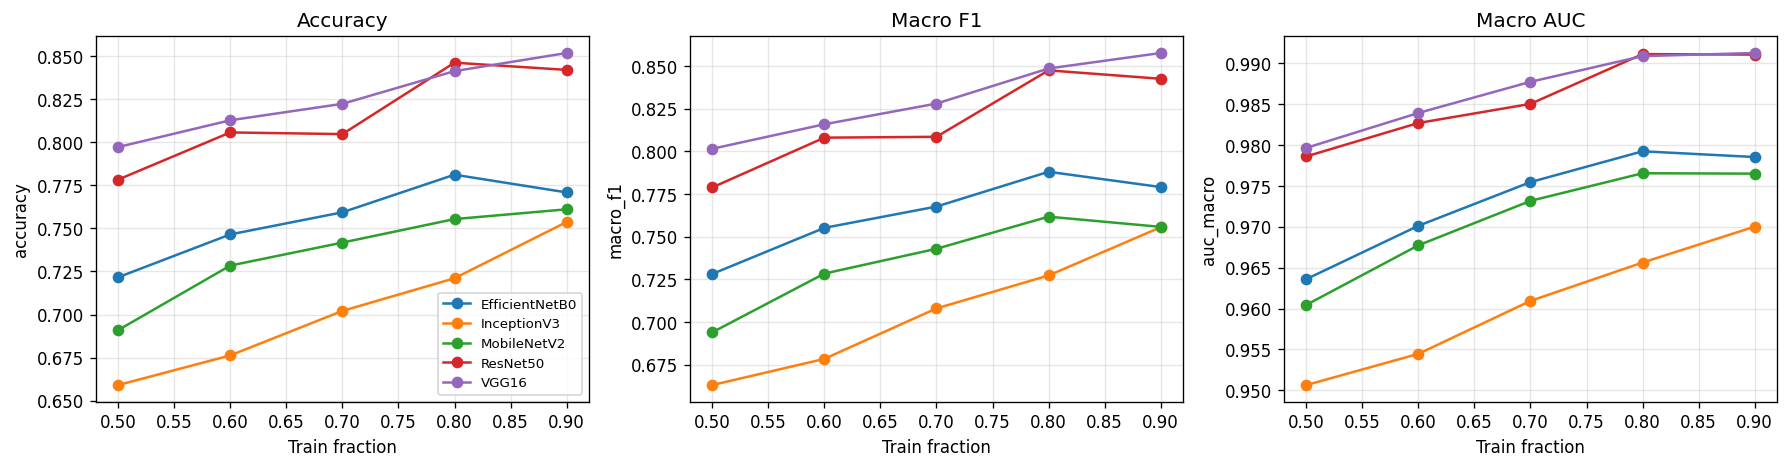
\includegraphics[width=\linewidth]{images/metrics_vs_split.png}
  \caption{Wpływ proporcji podziału train/test na accuracy, macro F1 i macro AUC. Każda krzywa odpowiada jednej architekturze.}
  \label{fig:metrics_vs_split}
\end{figure}

\subsection{Macierz pomyłek najlepszego modelu}

Macierz pomyłek dla najlepszego eksperymentu (VGG16, split 90/10) przedstawia Rys.~\ref{fig:cm_best}. Na przekątnej widoczne są wartości znacząco większe niż poza nią, co potwierdza skuteczność klasyfikatora. Najwyraźniej zaznacza się pomyłka między kartami \textit{six} oraz \textit{nine}, co odpowiada symetrii obrotowej tych cyfr (po obrocie o 180\textdegree{} wyglądają niemal identycznie). Pozostałe pomyłki rozkładają się równomiernie i mają znacznie mniejszą intensywność.

\begin{figure}[h!]
  \centering
  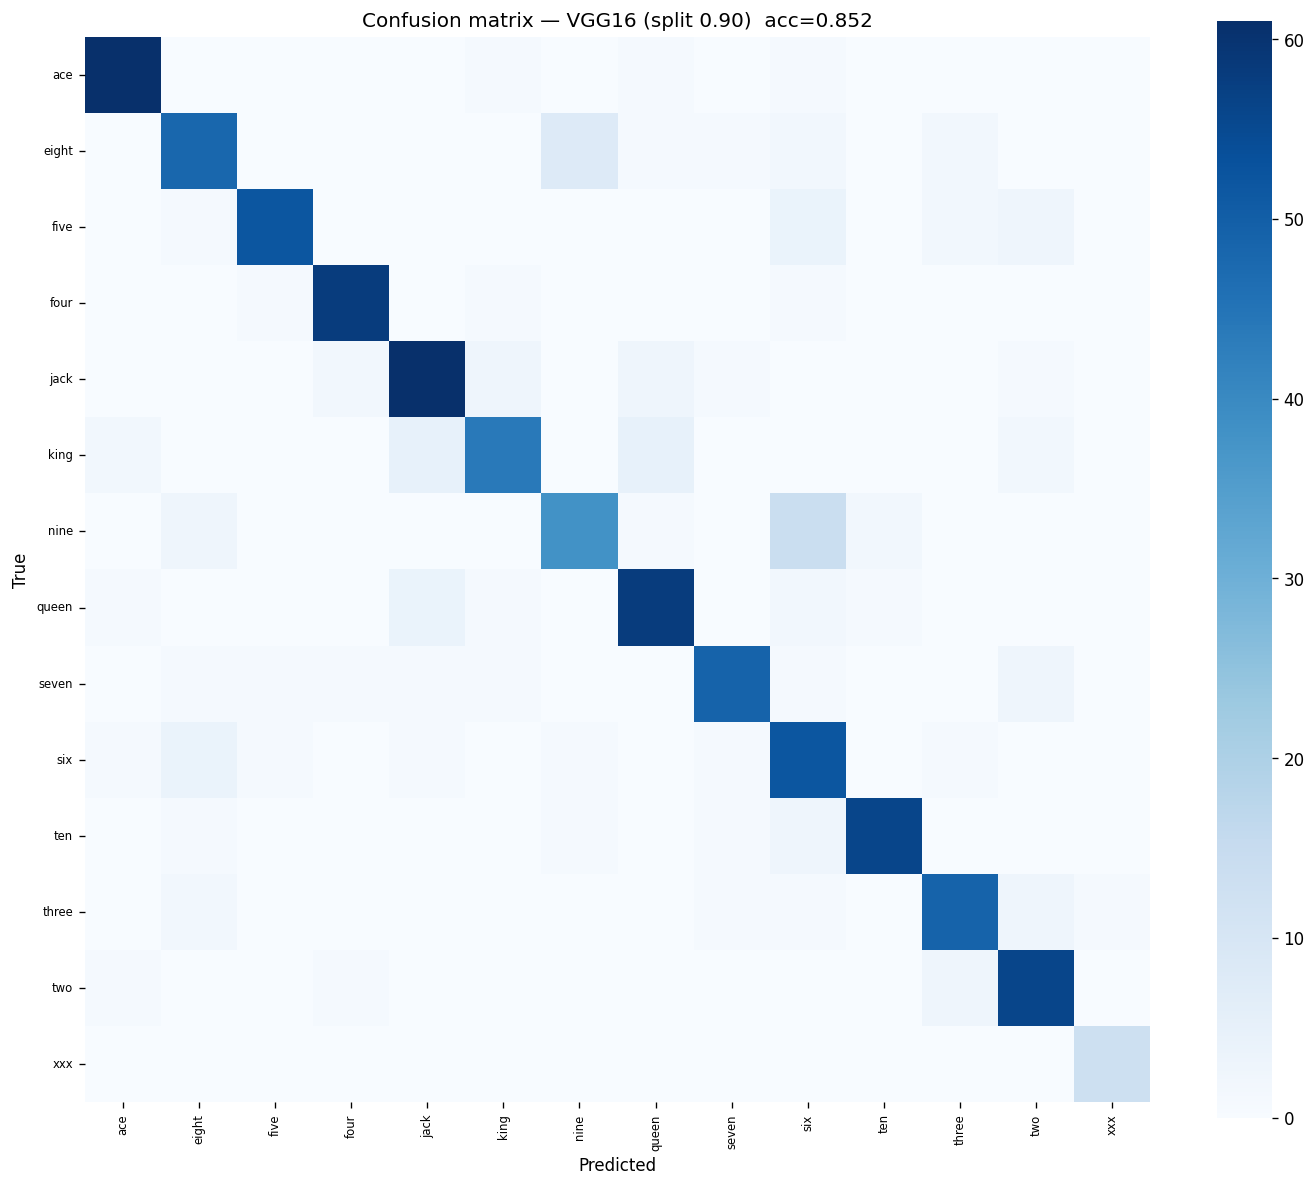
\includegraphics[width=0.85\linewidth]{images/cm_VGG16_90.png}
  \caption{Macierz pomyłek dla modelu VGG16 przy podziale 90/10.}
  \label{fig:cm_best}
\end{figure}

\subsection{Krzywe ROC najlepszego modelu}

Krzywe ROC w wariancie one-vs-rest dla pięciu najtrudniejszych i pięciu najłatwiejszych klas najlepszego modelu prezentuje Rys.~\ref{fig:roc_best}. Wszystkie krzywe znajdują się znacząco powyżej linii losowego klasyfikatora, a wartości AUC dla większości klas przekraczają 0{,}97.

\begin{figure}[h!]
  \centering
  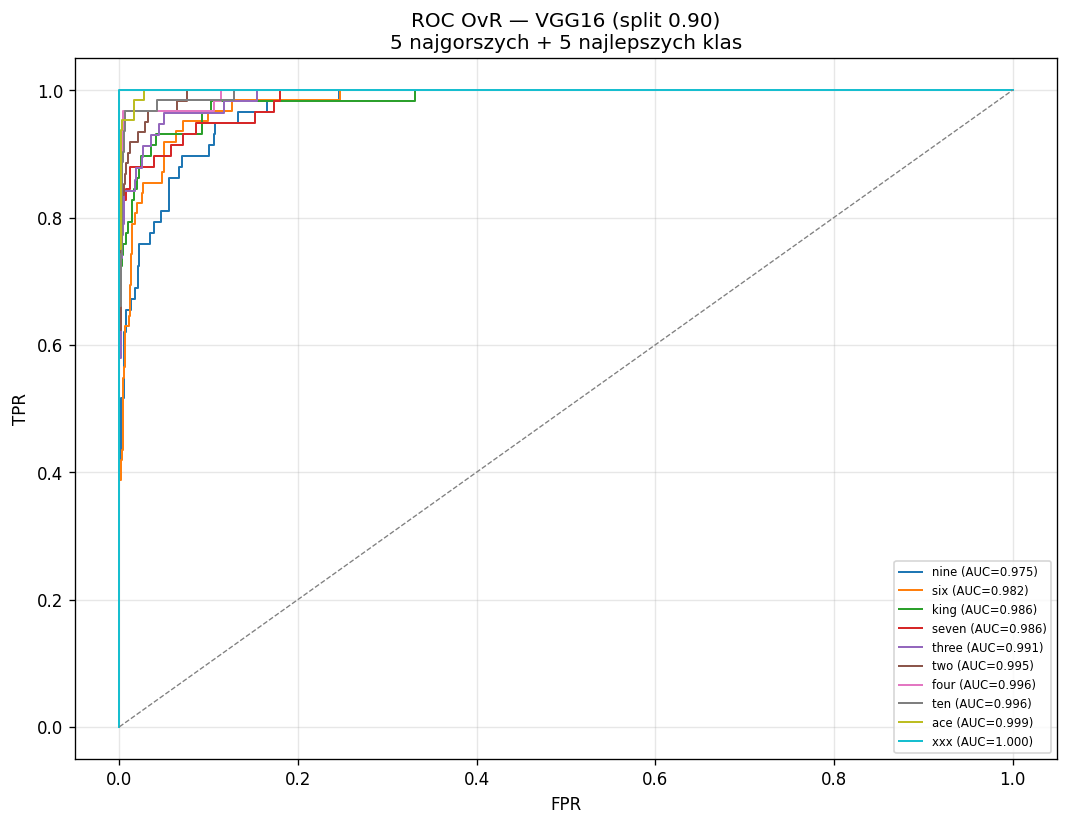
\includegraphics[width=0.85\linewidth]{images/roc_VGG16_90.png}
  \caption{Krzywe ROC OvR dla VGG16 przy podziale 90/10 -- pięć klas o najniższym i najwyższym AUC.}
  \label{fig:roc_best}
\end{figure}

\subsection{Krzywe uczenia}

Przebiegi funkcji straty oraz accuracy w trakcie treningu wszystkich 25 eksperymentów przedstawia Rys.~\ref{fig:learning}. Dla każdej architektury widoczna jest charakterystyczna dwuetapowość -- wyraźny spadek straty na początku fazy 2 (gdy odmrożenie warstw umożliwia dostrojenie ekstraktora cech do dziedziny kart).

\begin{figure}[h!]
  \centering
  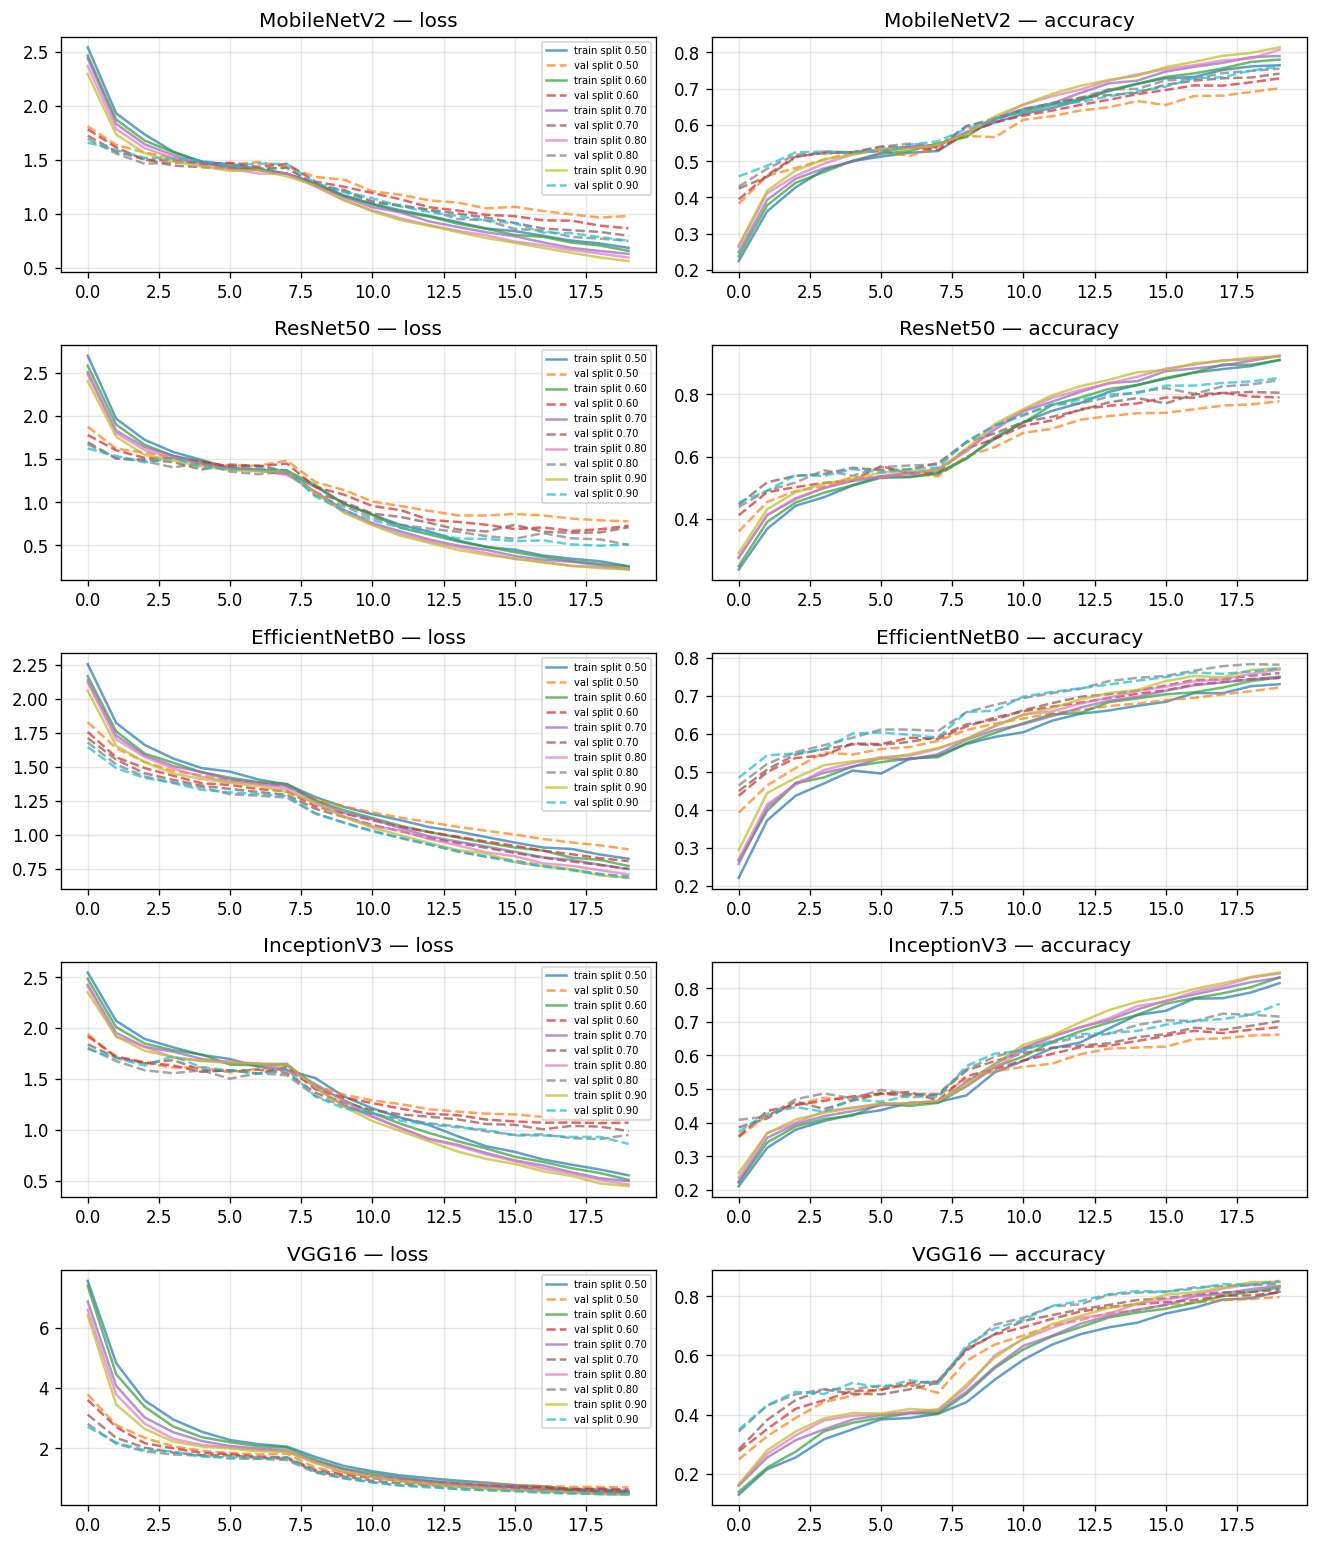
\includegraphics[width=\linewidth]{images/learning_curves.png}
  \caption{Krzywe uczenia (strata oraz accuracy) dla wszystkich modeli i podziałów.}
  \label{fig:learning}
\end{figure}

\FloatBarrier

%%%%%%%%%%%%%%%%%%%%%%%%%%%%%%%%%%%%%%%%%%%%%%%%%%%%%%%%%%%%%%%%%%%%%%%%%%%%%%%%
\section{Wnioski}

\begin{enumerate}
  \item Procedura treningu okazała się czynnikiem znacznie istotniejszym niż wybór konkretnej architektury. Trening wyłącznie głowy klasyfikującej dawał dla wszystkich modeli zbliżone wyniki (38--52\% accuracy), niezależnie od liczby parametrów; dopiero wprowadzenie fazy fine-tuningu pozwoliło ujawnić rzeczywiste różnice jakościowe między architekturami.

  \item Dobór augmentacji wymaga uwzględnienia specyfiki dziedziny. Powszechnie stosowane odbicie poziome (\texttt{RandomFlip}) okazało się szkodliwe ze względu na zorientowany charakter obrazów kart, podczas gdy augmentacja kolorystyczna (jasność, kontrast) przyniosła wyraźną poprawę ze względu na stylistyczną różnorodność źródeł obrazów w zbiorze.

  \item Granularność problemu wpływa na jakość znacznie silniej niż wybór modelu. Redukcja liczby klas z 53 do 14 typów (przy zachowaniu tego samego zbioru) podniosła accuracy o około 15 punktów procentowych, jednocześnie ujawniając czytelniejszą hierarchię modeli. Sugeruje to, że w problemach z ograniczoną liczbą próbek na klasę warto rozważyć agregację klas o ile pozwala na to definicja zadania.

  \item Wartości AUC \textit{macro} przekraczające 0{,}95 przy accuracy w przedziale 0{,}66--0{,}85 wskazują, że modele poprawnie szeregują klasy nawet wtedy, gdy ostateczna predykcja \textit{top-1} jest błędna. Dla zastosowań akceptujących wskazanie kilku najbardziej prawdopodobnych klas praktyczna skuteczność jest istotnie wyższa niż sugeruje samo accuracy.

  \item Nowsze architektury nie zawsze przewyższają starsze. Najwyższe wyniki osiągnęły VGG16 (2014) oraz ResNet50 (2015), podczas gdy EfficientNetB0 (2019) uzyskał wyniki średnie. Dowodzi to, że benchmarki na dużych zbiorach obrazów naturalnych nie przenoszą się wprost na dziedziny o specyficznym charakterze wizualnym.

  \item Wpływ proporcji podziału jest monotoniczny w zakresie 50/50--80/20, jednak przy podziale 90/10 obserwowana jest zwiększona wariancja estymaty wynikająca z małej liczebności zbioru testowego. W badaniach wymagających większej precyzji oszacowania wskazane byłoby zastosowanie walidacji krzyżowej.

  \item Wykorzystanie bardzo nowej generacji sprzętu (RTX 5080, architektura Blackwell) wymagało użycia najnowszej wersji TensorFlow oraz wiązało się z incydentalnymi problemami stabilności narzędzi w warstwie kompilacji XLA. Warto uwzględnić ten aspekt przy planowaniu podobnych eksperymentów -- dojrzałość ekosystemu sprzętowego bywa równie istotna co jego wydajność.
\end{enumerate}

%%%%%%%%%%%%%%%%%%%%%%%%%%%%%%%%%%%%%%%%%%%%%%%%%%%%%%%%%%%%%%%%%%%%%%%%%%%%%%%%
\renewcommand\refname{Bibliografia}
\bibliographystyle{plain}
\bibliography{bibliografia}

\end{document}
